\documentclass[border=2pt]{standalone}
\usepackage{pgfplots}\pgfplotsset{compat=1.18}\usepackage{amsmath}
\begin{document}
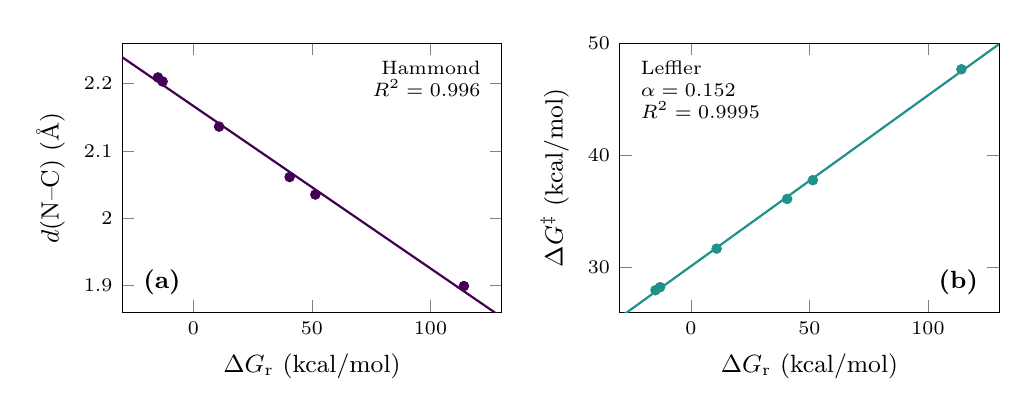
\begin{tikzpicture}
  \definecolor{c1}{HTML}{440154}\definecolor{c2}{HTML}{21918C}\definecolor{c3}{HTML}{E1A800}
  \pgfplotsset{every axis/.append style={width=6.4cm,height=5cm,
    tick label style={font=\scriptsize},label style={font=\small},
    tick align=inside,mark size=1.7pt}}

  \begin{axis}[name=a,
      xlabel={$\Delta G_\mathrm{r}$ (kcal/mol)}, ylabel={$d$(N--C) (\AA)},
      xmin=-30, xmax=130, ymin=1.86, ymax=2.26, xtick={0,50,100}]
    \addplot[c1, thick, domain=-30:130, forget plot] {-0.002414*x + 2.1666};
    \addplot[only marks, mark=*, c1, forget plot] coordinates {
      (114.09,1.899) (51.43,2.035) (40.59,2.061)
      (10.85,2.136) (-12.97,2.203) (-14.93,2.209)};
    \node[font=\scriptsize, anchor=north east, align=right] at (rel axis cs:0.97,0.97)
      {Hammond\\$R^2 = 0.996$};
    \node[font=\small\bfseries, anchor=south west] at (rel axis cs:0.03,0.03) {(a)};
  \end{axis}

  \begin{axis}[at={(a.east)}, anchor=west, xshift=1.5cm,
      xlabel={$\Delta G_\mathrm{r}$ (kcal/mol)},
      ylabel={$\Delta G^\ddagger$ (kcal/mol)},
      xmin=-30, xmax=130, ymin=26, ymax=50, xtick={0,50,100}]
    \addplot[c2, thick, domain=-30:130, forget plot] {0.152394*x + 30.1064};
    \addplot[only marks, mark=*, c2, forget plot] coordinates {
      (114.09,47.67) (51.43,37.78) (40.59,36.11)
      (10.85,31.68) (-12.97,28.24) (-14.93,27.97)};
    \node[font=\scriptsize, anchor=north west, align=left] at (rel axis cs:0.03,0.97)
      {Leffler\\$\alpha = 0.152$\\$R^2 = 0.9995$};
    \node[font=\small\bfseries, anchor=south east] at (rel axis cs:0.97,0.03) {(b)};
  \end{axis}
\end{tikzpicture}
\end{document}
